\documentclass[a4paper]{article}

\usepackage[pdftex,
  hidelinks,
  pdfauthor={Dexter Chua},
  pdfsubject={Cambridge Maths Notes: Part IA - Probability},
  pdftitle={Part IA - Probability},
pdfkeywords={Cambridge Mathematics Maths Math IA Lent Probability}]{hyperref}

% Imports
\ifx \nextra \undefined
  \usepackage[pdftex,
    hidelinks,
    pdfauthor={Dexter Chua},
    pdfsubject={Cambridge Maths Notes: Part \npart\ - \ncourse},
    pdftitle={Part \npart\ - \ncourse},
  pdfkeywords={Cambridge Mathematics Maths Math \npart\ \nterm\ \nyear\ \ncourse}]{hyperref}
  \title{Part \npart\ - \ncourse}
\else
  \usepackage[pdftex,
    hidelinks,
    pdfauthor={Dexter Chua},
    pdfsubject={Cambridge Maths Notes: Part \npart\ - \ncourse\ (\nextra)},
    pdftitle={Part \npart\ - \ncourse\ (\nextra)},
  pdfkeywords={Cambridge Mathematics Maths Math \npart\ \nterm\ \nyear\ \ncourse\ \nextra}]{hyperref}

  \title{Part \npart\ - \ncourse \\ {\Large \nextra}}
\fi

\author{Lectured by \nlecturer \\\small Notes taken by Dexter Chua}
\date{\nterm\ \nyear}

\usepackage{alltt}
\usepackage{amsfonts}
\usepackage{amsmath}
\usepackage{amssymb}
\usepackage{amsthm}
\usepackage{booktabs}
\usepackage{caption}
\usepackage{enumitem}
\usepackage{fancyhdr}
\usepackage{graphicx}
\usepackage{mathtools}
\usepackage{microtype}
\usepackage{multirow}
\usepackage{pdflscape}
\usepackage{pgfplots}
\usepackage{siunitx}
\usepackage{tabularx}
\usepackage{tikz}
\usepackage{tkz-euclide}
\usepackage[normalem]{ulem}
\usepackage[all]{xy}

\pgfplotsset{compat=1.12}

\pagestyle{fancyplain}
\lhead{\emph{\nouppercase{\leftmark}}}
\ifx \nextra \undefined
  \rhead{
    \ifnum\thepage=1
    \else
      \npart\ \ncourse
    \fi}
\else
  \rhead{
    \ifnum\thepage=1
    \else
      \npart\ \ncourse\ (\nextra)
    \fi}
\fi
\usetikzlibrary{arrows}
\usetikzlibrary{decorations.markings}
\usetikzlibrary{decorations.pathmorphing}
\usetikzlibrary{positioning}
\usetikzlibrary{fadings}
\usetikzlibrary{intersections}
\usetikzlibrary{cd}

\newcommand*{\Cdot}{\raisebox{-0.25ex}{\scalebox{1.5}{$\cdot$}}}
\newcommand {\pd}[2][ ]{
  \ifx #1 { }
    \frac{\partial}{\partial #2}
  \else
    \frac{\partial^{#1}}{\partial #2^{#1}}
  \fi
}

% Theorems
\theoremstyle{definition}
\newtheorem*{aim}{Aim}
\newtheorem*{axiom}{Axiom}
\newtheorem*{claim}{Claim}
\newtheorem*{cor}{Corollary}
\newtheorem*{defi}{Definition}
\newtheorem*{eg}{Example}
\newtheorem*{fact}{Fact}
\newtheorem*{law}{Law}
\newtheorem*{lemma}{Lemma}
\newtheorem*{notation}{Notation}
\newtheorem*{prop}{Proposition}
\newtheorem*{thm}{Theorem}

\renewcommand{\labelitemi}{--}
\renewcommand{\labelitemii}{$\circ$}
\renewcommand{\labelenumi}{(\roman{*})}

\let\stdsection\section
\renewcommand\section{\newpage\stdsection}

% Strike through
\def\st{\bgroup \ULdepth=-.55ex \ULset}

% Maths symbols
\newcommand{\bra}{\langle}
\newcommand{\ket}{\rangle}

\newcommand{\N}{\mathbb{N}}
\newcommand{\Z}{\mathbb{Z}}
\newcommand{\Q}{\mathbb{Q}}
\renewcommand{\H}{\mathbb{H}}
\newcommand{\R}{\mathbb{R}}
\newcommand{\C}{\mathbb{C}}
\newcommand{\Prob}{\mathbb{P}}
\renewcommand{\P}{\mathbb{P}}
\newcommand{\E}{\mathbb{E}}
\newcommand{\F}{\mathbb{F}}
\newcommand{\cU}{\mathcal{U}}
\newcommand{\RP}{\mathbb{RP}}
\newcommand{\CP}{\mathbb{CP}}

\newcommand{\ph}{\,\cdot\,}

\DeclareMathOperator{\sech}{sech}
\DeclareMathOperator{\cosech}{cosech}
\DeclareMathOperator{\cosec}{cosec}

\DeclareMathOperator{\covol}{covol}
\DeclareMathOperator{\vol}{vol}

\let\Im\relax
\let\Re\relax
\DeclareMathOperator{\Im}{Im}
\DeclareMathOperator{\Re}{Re}
\DeclareMathOperator{\im}{im}
\DeclareMathOperator{\image}{image}
\DeclareMathOperator{\Ann}{Ann}

\DeclareMathOperator*{\res}{res}
\DeclareMathOperator{\Res}{Res}
\DeclareMathOperator{\Ind}{Ind}

\DeclareMathOperator{\tr}{tr}
\DeclareMathOperator{\diag}{diag}
\DeclareMathOperator{\rank}{rank}
\DeclareMathOperator{\card}{card}
\DeclareMathOperator{\spn}{span}
\DeclareMathOperator{\adj}{adj}

\DeclareMathOperator{\erf}{erf}
\DeclareMathOperator{\erfc}{erfc}

\DeclareMathOperator{\ord}{ord}
\DeclareMathOperator{\Sym}{Sym}

\DeclareMathOperator{\sgn}{sgn}
\DeclareMathOperator{\orb}{orb}
\DeclareMathOperator{\stab}{stab}
\DeclareMathOperator{\ccl}{ccl}

\DeclareMathOperator{\lcm}{lcm}
\DeclareMathOperator{\hcf}{hcf}

\DeclareMathOperator{\Int}{Int}
\DeclareMathOperator{\id}{id}

\DeclareMathOperator{\betaD}{beta}
\DeclareMathOperator{\gammaD}{gamma}
\DeclareMathOperator{\Poisson}{Poisson}
\DeclareMathOperator{\binomial}{binomial}
\DeclareMathOperator{\multinomial}{multinomial}
\DeclareMathOperator{\Bernoulli}{Bernoulli}
\DeclareMathOperator{\like}{like}

\DeclareMathOperator{\var}{var}
\DeclareMathOperator{\cov}{cov}
\DeclareMathOperator{\bias}{bias}
\DeclareMathOperator{\mse}{mse}
\DeclareMathOperator{\corr}{corr}

\DeclareMathOperator{\otp}{otp}
\DeclareMathOperator{\dom}{dom}

\DeclareMathOperator{\Root}{Root}
\DeclareMathOperator{\supp}{supp}
\DeclareMathOperator{\rel}{rel}
\DeclareMathOperator{\Hom}{Hom}
\DeclareMathOperator{\Aut}{Aut}
\DeclareMathOperator{\Gal}{Gal}
\DeclareMathOperator{\Mat}{Mat}
\DeclareMathOperator{\End}{End}
\DeclareMathOperator{\Char}{char}
\DeclareMathOperator{\ev}{ev}
\DeclareMathOperator{\St}{St}
\DeclareMathOperator{\Lk}{Lk}
\DeclareMathOperator{\disc}{disc}
\DeclareMathOperator{\Isom}{Isom}
\DeclareMathOperator{\length}{length}
\DeclareMathOperator{\energy}{energy}
\DeclareMathOperator{\area}{area}
\DeclareMathOperator{\Syl}{Syl}
\DeclareMathOperator{\cl}{cl}
\DeclareMathOperator{\fix}{fix}

\newcommand{\GL}{\mathrm{GL}}
\newcommand{\SL}{\mathrm{SL}}
\newcommand{\PGL}{\mathrm{PGL}}
\newcommand{\PSL}{\mathrm{PSL}}
\newcommand{\PSU}{\mathrm{PSU}}
\newcommand{\Or}{\mathrm{O}}
\newcommand{\SO}{\mathrm{SO}}
\newcommand{\U}{\mathrm{U}}
\newcommand{\SU}{\mathrm{SU}}

\renewcommand{\d}{\mathrm{d}}
\newcommand{\D}{\mathrm{D}}

\tikzset{->/.style = {decoration={markings,
                                  mark=at position 1 with {\arrow[scale=2]{latex'}}},
                      postaction={decorate}}}
\tikzset{<-/.style = {decoration={markings,
                                  mark=at position 0 with {\arrowreversed[scale=2]{latex'}}},
                      postaction={decorate}}}
\tikzset{<->/.style = {decoration={markings,
                                   mark=at position 0 with {\arrowreversed[scale=2]{latex'}},
                                   mark=at position 1 with {\arrow[scale=2]{latex'}}},
                       postaction={decorate}}}
\tikzset{->-/.style = {decoration={markings,
                                   mark=at position #1 with {\arrow[scale=2]{latex'}}},
                       postaction={decorate}}}
\tikzset{-<-/.style = {decoration={markings,
                                   mark=at position #1 with {\arrowreversed[scale=2]{latex'}}},
                       postaction={decorate}}}

\tikzset{circ/.style = {fill, circle, inner sep = 0, minimum size = 3}}
\tikzset{mstate/.style={circle, draw, blue, text=black, minimum width=0.7cm}}

\definecolor{mblue}{rgb}{0.2, 0.3, 0.8}
\definecolor{morange}{rgb}{1, 0.5, 0}
\definecolor{mgreen}{rgb}{0.1, 0.4, 0.2}
\definecolor{mred}{rgb}{0.5, 0, 0}

\def\drawcirculararc(#1,#2)(#3,#4)(#5,#6){%
    \pgfmathsetmacro\cA{(#1*#1+#2*#2-#3*#3-#4*#4)/2}%
    \pgfmathsetmacro\cB{(#1*#1+#2*#2-#5*#5-#6*#6)/2}%
    \pgfmathsetmacro\cy{(\cB*(#1-#3)-\cA*(#1-#5))/%
                        ((#2-#6)*(#1-#3)-(#2-#4)*(#1-#5))}%
    \pgfmathsetmacro\cx{(\cA-\cy*(#2-#4))/(#1-#3)}%
    \pgfmathsetmacro\cr{sqrt((#1-\cx)*(#1-\cx)+(#2-\cy)*(#2-\cy))}%
    \pgfmathsetmacro\cA{atan2(#2-\cy,#1-\cx)}%
    \pgfmathsetmacro\cB{atan2(#6-\cy,#5-\cx)}%
    \pgfmathparse{\cB<\cA}%
    \ifnum\pgfmathresult=1
        \pgfmathsetmacro\cB{\cB+360}%
    \fi
    \draw (#1,#2) arc (\cA:\cB:\cr);%
}
\newcommand\getCoord[3]{\newdimen{#1}\newdimen{#2}\pgfextractx{#1}{\pgfpointanchor{#3}{center}}\pgfextracty{#2}{\pgfpointanchor{#3}{center}}}

\def\Xint#1{\mathchoice
   {\XXint\displaystyle\textstyle{#1}}%
   {\XXint\textstyle\scriptstyle{#1}}%
   {\XXint\scriptstyle\scriptscriptstyle{#1}}%
   {\XXint\scriptscriptstyle\scriptscriptstyle{#1}}%
   \!\int}
\def\XXint#1#2#3{{\setbox0=\hbox{$#1{#2#3}{\int}$}
     \vcenter{\hbox{$#2#3$}}\kern-.5\wd0}}
\def\ddashint{\Xint=}
\def\dashint{\Xint-}


\title{Part IA - Probability}
\author{Lectured by R. Weber}
\date{Lent 2015}

\begin{document}
\maketitle
{\small
  \noindent\textbf{Basic concepts}\\
  Classical probability, equally likely outcomes. Combinatorial analysis, permutations and combinations.  Stirling's formula (asymptotics for $\log n!$ proved).\hspace*{\fill}  [3]
 
  \vspace{10pt}
  \noindent\textbf{Axiomatic approach}\\
  Axioms (countable case). Probability spaces. Inclusion-exclusion formula. Continuity and subadditivity of probability measures. Independence. Binomial, Poisson and geometric distributions. Relation between Poisson and binomial distributions. Conditional probability, Bayes's formula. Examples, including Simpson's paradox.\hspace*{\fill} [5]
 
  \vspace{10pt}
  \noindent\textbf{Discrete random variables}\\
  Expectation. Functions of a random variable, indicator function, variance, standard deviation. Covariance, independence of random variables. Generating functions: sums of independent random variables, random sum formula, moments.
 
  \vspace{5pt}
  \noindent Conditional expectation. Random walks: gambler's ruin, recurrence relations. Difference equations and their solution. Mean time to absorption. Branching processes: generating functions and extinction probability. Combinatorial applications of generating functions.\hspace*{\fill} [7]
 
  \vspace{10pt}
  \noindent\textbf{Continuous random variables}\\
  Distributions and density functions. Expectations; expectation of a function of a random variable.  Uniform, normal and exponential random variables. Memoryless property of exponential distribution.  Joint distributions: transformation of random variables (including Jacobians), examples. Simulation: generating continuous random variables, independent normal random variables. Geometrical probability: Bertrand's paradox, Buffon's needle. Correlation coefficient, bivariate normal random variables.\hspace*{\fill} [6]
 
  \vspace{10pt}
  \noindent\textbf{Inequalities and limits}\\
  Markov's inequality, Chebyshev's inequality. Weak law of large numbers. Convexity: Jensen's inequality for general random variables, AM/GM inequality.
 
  \vspace{5pt}
  \noindent Moment generating functions and statement (no proof) of continuity theorem. Statement of central limit theorem and sketch of proof. Examples, including sampling.\hspace*{\fill} [3]}


\tableofcontents
\setcounter{section}{-1}
\section{Introduction}
In every day life, we often encounter the use of the term probability, and they are used in many different ways. For example, we can hear people say:
\begin{enumerate}
  \item The probability that a fair coin will land heads is $1/2$.
  \item The probability that a selection of 6 members wins the National Lottery Lotto jackpot is 1 in $\binom{19}{6} = 13 983 816$ or $7.15112\times 10^{-8}$.
  \item The probability that a drawing pin will land 'point up' is 0.62.
  \item The probabilty that a large earthquake will occur on the San Andreas Fault in the next 30 years is about $21\%$
  \item The probability that humanity will be extinct by 2100 is about $50\%$
\end{enumerate}
The first two cases are things derived from logic. We know that the coin either lands heads or tails. By definition, a fair coin is equally likely to land heads or tail. So the probability of either must be $1/2$.

The third is something probably derived from experiments. Perhaps we did 1000 experiments and 620 of the pins point up. The fourth and fifth examples belong to yet another category that talks about are beliefs and predictions.

We call the first kind ``classical probability'', the second kind ``frequentist probability'' and the last ``subjective probability''. In this course, we only consider classical probability.

\section{Classical probability}
\subsection{Classical probability}
\begin{defi}[Classical probability]
  \emph{Classical probability} applies in a situation when there are a finite number of equally likely outcome.
\end{defi}

Consider the problem of points

$A$ and $B$ play a game in which they keep throwing coins. If a head lands, then $A$ gets a point. Otherwise, $B$ gets a point. The first person to get 10 points wins a prize.

Now suppose $A$ has got 8 points and $B$ has got 7. The game has to end because an earthquake struck. How should they divide the prize? We answer this by finding the probability of $A$ winning. Someone must have won by the end of 19 rounds, i.e. after 4 more rounds. If $A$ wins at least 2 of them, then $A$ wins.

The number of ways this can happen is $\binom{4}{2} + \binom{4}{3} + \binom{4}{4} = 11$. So $A$ should get $11/16$ of the prize.

\subsection{Sample space and events}
Consider an experiment that has a random outcome.

\begin{defi}[Sample space]
  The set of all possible outcomes is the \emph{sample space}, $\Omega$. We can lists the outcomes as $\omega_1, \omega_2, \cdots \in \Omega$. Each $\omega \in \Omega$ is an \emph{outcome}.
\end{defi}

\begin{defi}[Event]
  A subset of $\Omega$ is called an \emph{event}.
\end{defi}

\begin{defi}[Set notations]
  Given any two events $A, B\subseteq \Omega$,
  \begin{itemize}
    \item The \emph{complement} of $A$ is $A^C = A' = \bar A = \omega\setminus A$.
    \item ``$A$ or $B$'' is the set $A\cup B$.
    \item ``$A$ and $B$''  is the set $A\cap B$.
    \item $A$ and $B$ are \emph{mutually exclusive} or \emph{disjoint} if $A\cap B = \emptyset$.
    \item $A\subseteq B$ means $A\Rightarrow B$.
  \end{itemize}
\end{defi}

\begin{defi}[Probability]
  Suppose $\Omega = \{\omega_1,\omega_2, \cdots, \omega_N\}$. Let $A\subseteq \Omega$ be an event. Then the \emph{probability} of $A$ is
  \[
    P(A) = \frac{\text{Number of outcomes in } A}{\text{Number of outcomes in }\omega} = \frac{|A|}{N}
  \]
\end{defi}

\begin{eg}
  Suppose $r$ digits are drawn at random from a table of random digits from 0 to 9. What is the probability of
  \begin{enumerate}
    \item No digit exceeds $k$
    \item The largest digit drawn is $k$
  \end{enumerate}

  The sample space is $\Omega = \{(a_1, a_2, \cdots, a_r): 0 \leq a_i \leq 9\}$. Then $|\Omega| = 10^r$.

  Let $A_k = [\text{no digit exceeds }k] = \{(a_1, \cdots, a_r): 0 \leq a_i \leq k\}$. Then $|A_k| = (k + 1)^r$. So $P(A_k) = (k + 1)^r/10^r$.

  Now let $B_k = [\text{largest digit drawn is k}]$. We can find this by finding all outcomes in which no digits exceed $k$, and subtract it by the number of outcomes in which no digit exceeds $k - 1$. So $|B_k| = |A_k| - |A_{k - 1}|$ and $P(B_k) = [(k + 1)^r - k^r]/10^r$.
\end{eg}

\section{Combinatorial analysis}
\subsection{Counting}
\begin{eg}
  A menu has 6 starters, 7 mains and 6 desserts. How many meals are there? Clearly $6 \times 7 \times 6 = 252$.
\end{eg}
This is the fundamental rule of counting:
\begin{thm}[Fundamental rule of counting]
  Suppose we have to make $r$ multiple choices in sequence. There are $m_1$ possibilities for the first choice, $m_2$ possibilities for the second etc. Then the total number of choices is $m_1\times m_2\times \cdots m_r$.
\end{thm}

\begin{eg}
  How many ways can $1, 2, \cdots, n$ be ordered? The first choice has $n$ possibilities, the second has $n - 1$ possibilities etc. So there are $n\times (n - 1)\times\cdots \times 1 = n!$.
\end{eg}

\subsection{Sampling with or without replacement}
Let $N = \{1, 2, \cdots, n\}$ be a list. Let $X = \{1, 2, \cdots, x\}$ be the items. Let $f: N\to X$ with $f(i) =$ item at the $i$th position.

\begin{defi}[1. Sampling with replacement]
  When we sample with replacement, after choosing at item, it is put back and can be chosen again. Then any sampling function $f$ satisfies sampling with replacement.
\end{defi}

\begin{defi}[2. Sampling without replacement]
  After choosing an item, we burn it and cannot choose it again. Then $f$ must be an injective function, and clearly we must have $X \geq n$.
\end{defi}

We can also have sampling with replacement, but we require each item to be chosen at least once. In this case, $f$ must be surjective.

\begin{eg}
  Suppose $N = \{a, b, c\}$ and $X = \{p, q, r, s\}$. How many injective functions are there $N\to X$?

  When we choose $f(a)$, we have 4 options. When we choose $f(b)$, we have 3 left. When we choose $f(c)$, we have 2 choices left. So there are $24$ possible choices.
\end{eg}

\begin{eg}
  I have $n$ keys in my pocket. We select one at random once and try to unlock. What is the possibility that I succeed at the $r$th trial?

  Suppose we do it with replacement. We have to fail the first $r - 1$ trials and succeed in the $r$th. So The probability is
  \[
    \frac{(n - 1)(n - 1) \cdots (n - 1)(1)}{n^r} = \frac{(n - 1)^{r - 1}}{n^r}.
  \]
  Now suppose we are smarter and try without replacement. Then the probability is
  \[
    \frac{(n - 1)(n - 2)\cdots (n - r + 1)(1)}{n(n - 1) \cdots (n - r + 1)} = \frac{1}{n}.
  \]
\end{eg}
\begin{eg}[Birthday problem]
  How many people are needed in a room for there to be a probability of at least a half that two people have the same birthday?

  Suppose $f(r)$ is the probability that, in a room of $r$ people, there is a birthday match.

  We solve this by finding the probability of no match, $1 - f(r)$. The total number of possibilities of birthday combinations is $365^r$. For nobody to have the same birthday, the first person can have any birthday. The second has 364 else to choose, etc.
  \[
    P(\text{no match}) = \frac{365\cdot 364\cdot 363 \cdots (366 - r)}{365\cdot 365\cdot 365 \cdots 365}
  \]
  If we calculate this with a computer, we find that $f(22) = 0.475695$ and $f(23) = 0.507297$.

  While this might sound odd since 23 is small, we shouldn't be counting the number of people, but the number of pairs. With 23 people, we have $23\times 22/2 = 253$ pairs, which is quite large compared to 365.
\end{eg}
\subsection{Sampling with or without regard to ordering}
Do the labels on the list positions or items matter?

Recall we have the function $f: N\to X$ and they map $f(1), f(2), \cdots, f(n)$.

After choosing the numbers, we can
\begin{itemize}
  \item Leave the list alone
  \item Sort the list ascending. i.e. we might get $(2, 5, 4)$ and $(4, 2, 5)$. If we don't care about list positions, these are just equivalent to $(2, 4, 5)$.
  \item Re-number each item by the number of the draw on which it was first seen. For example, we can rename $(2, 5, 2)$ and $(5, 4, 5)$ both as $(1, 2, 1)$. This happens if the labelling of items doesn't matter.
  \item Both of above. So we can rename $(2, 5, 2)$ and $(8, 5, 5)$ both as $(1, 1, 2)$.
\end{itemize}

Combining these four possibilities with whether we have replacement or not, we have 12 possible cases of counting.

\subsection{Four cases of enumerative combinatorics}
\begin{itemize}
  \item Replacement + with ordering: the number of ways is $x^n$.
  \item Without replacement + with ordering: the number of ways is $x_{(n)} = x^{\underline{n}} = x(x - 1)\cdots (x - n + 1)$.
  \item Without replacement + without order: we only care which items get selected. The number of ways is $\binom{x}{n} = C^x_n = x_{(n)}/n!$.
  \item Replacement + without ordering: we only care how many times the item got chosen. We want to find ways to partition $n = n_1 + n_2 + \cdots n_x$. Say $n = 6$ and $x = 3$. We can write a particular partition as
    \[
      **|*|***
    \]
  So we have $n + x - 1$ symbols and $x - 1$ of them are bars. So the number of ways is $\binom{n + x - 1}{x - 1}$.
\end{itemize}
\section{Stirling's formula}
\subsection{Multinomial coefficient}
Suppose we fill successive positions in a list of length $n$, with replacement, from a set of $x$ items. How many ways can this be done so that item $i\in X$ is used $n_i$ times? (of course we must have $n_1 + n_2 + \cdots + n_x = n$.

In the case of $x = 2$, we have the binomial coefficient. In general, we have
\begin{defi}[Multinomial coefficient]
  A \emph{multinomial coefficient} is
  \[
    \binom{n}{n_1, n_2, \cdots, n_x} = \binom{n}{n_1}\binom{n - n_1}{n_2}\cdots \binom{n - n_1\cdots - n_{x - 1}}{n_x} = \frac{n!}{n_1!n_2!\cdots n_x!}.
  \]
  It is the number of ways to distribute $x$ items into $n$ positions with replacement, in which the $i$th position has $n_i$ items.
\end{defi}

\begin{eg}
  We know that
  \[
    (x + y)^n = x^n + \binom{n}{1}x^{n - 1}y + \cdots + y^n.
  \]
  If we have a trinomial, then
  \[
    (x + y + z)^n = \sum_{n_1, n_2, n_3} \binom{n}{n_1, n_2, n_3} x^{n_1}y^{n_2}y^{n_3}.
  \]
\end{eg}

\begin{eg}
  How many ways can we deal 52 cards to 4 player, each with a hand of 13? There are
  \[
    \binom{52}{13, 13, 13, 13} = \frac{52!}{(13!)^4} = 53644737765488792839237440000 = 5.36\times 10^{28}.
  \]
\end{eg}
While computers are still capable of calculating that, what if we have more cards? Suppose each person has $n$ cards. Then the number of ways is
\[
  \frac{(4n)!}{(n!)^4} = \frac{2^{8n}}{\sqrt{2} (\pi n)^{3/2}}.
\]
We can use Stirling's Formula to approximate it:
\subsection{Stirling's formula}
Before we state and prove Stirling's formula, we prove a weaker (but examinable) version:
\begin{prop}
  $\log n!\sim n\log n$
\end{prop}
\begin{proof}
  Note that
  \[
    e^n = 1 + n + \frac{n^2}{2!} + \cdots + \frac{n^n}{n!} + \cdots.
  \]
  So $1 \leq n^n/n! \leq e^n$. Note that
  \[
    \log n! = \sum_{k=1}^n \log k.
  \]
  Now we claim that
  \[
    \int_1^n \log x\;\d x \leq \sum_1^n \log k\leq \int_1^{n + 1}\log x\;\d x.
  \]
  This is true by considering the diagram:
  \begin{center}
    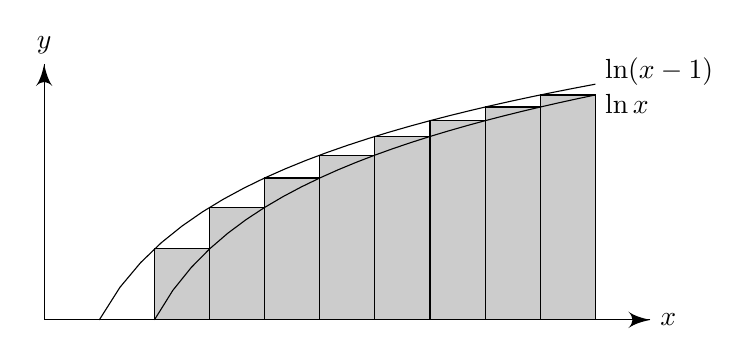
\begin{tikzpicture}[xscale=0.7, yscale=1.3]
     \draw [->] (0, 0) -- (11, 0) node [right] {$x$};
     \draw [->] (0, 0) -- (0, 2.5) node [above] {$y$};
     \draw [domain=2:10] plot (\x, {ln (\x - 1)}) node [anchor = south west] {$\ln (x - 1)$};
     \draw [domain=1:10] plot (\x, {ln \x }) node [anchor = north west] {$\ln x$};
     \draw [fill = black, fill opacity=0.2] (2, 0)-- (2, 0.693147180559945) -- (3, 0.693147180559945) -- (3, 0);
     \draw [fill = black, fill opacity=0.2] (3, 0)-- (3, 1.09861228866811) -- (4, 1.09861228866811) -- (4, 0);
     \draw [fill = black, fill opacity=0.2] (4, 0)-- (4, 1.38629436111989) -- (5, 1.38629436111989) -- (5, 0);
     \draw [fill = black, fill opacity=0.2] (5, 0)-- (5, 1.6094379124341) -- (6, 1.6094379124341) -- (6, 0);
     \draw [fill = black, fill opacity=0.2] (6, 0)-- (6, 1.79175946922806) -- (7, 1.79175946922806) -- (7, 0);
     \draw [fill = black, fill opacity=0.2] (7, 0)-- (7, 1.94591014905531) -- (8, 1.94591014905531) -- (8, 0);
     \draw [fill = black, fill opacity=0.2] (8, 0)-- (8, 2.07944154167984) -- (9, 2.07944154167984) -- (9, 0);
     \draw [fill = black, fill opacity=0.2] (9, 0)-- (9, 2.19722457733622) -- (10, 2.19722457733622) -- (10, 0);
    \end{tikzpicture}
  \end{center}
  Perform the integral to obtain
  \[
    n\log n - n + 1 \leq \log n! \leq (n+ 1)\log (n + 1) - n;
  \]
  Divide both sides by $n\log n$ and let $n\to \infty$. Both sides tend to $1$. So 
  \[
    \frac{\log n!}{n\log n} \to 1.
  \]
\end{proof}

Now we prove Stirling's Formula:
\begin{thm}[Stirling's formula]
  As $n\to \infty$,
  \[
    \log\left(\frac{n! e^n}{n^{n + \frac{1}{2}}}\right) = \log \sqrt{2\pi} + O\left(\frac{1}{n}\right)
  \]
\end{thm}
\begin{cor}
  \[
    n!\sim \sqrt{2\pi}n^{n + \frac{1}{2}} e^{-n}
  \]
\end{cor}
\begin{proof}(non-examinable)
  Define 
  \[
    d_n = \log \left(\frac{n!e^n}{n^{n + 1/2}}\right) = \log n! - (n + 1/2)\log n + n
  \]
  Then
  \[
    d_n - d_{n + 1} = (n + 1/2)\log\left(\frac{n + 1}{n}\right)
  \]
  Write $t = 1/(2n + 1)$. Then
  \[
    d_n - d_{n + 1} = \frac{1}{2t}\log\left(\frac{1 + t}{1 - t}\right).
  \]
  We can simplifying by noting that
  \begin{align*}
    \log (1 + t) - t &= -\frac{1}{2}t^2 + \frac{1}{3}t^3 - \frac{1}{4}t^4 + \cdots\\
    \log (1 - t) + t &= -\frac{1}{2}t^2 - \frac{1}{3}t^3 - \frac{1}{4}t^4 - \cdots
  \end{align*}
  Then if we subtract the equations and divide by $2t$, we obtain
  \begin{align*}
    d_n - d_{n + 1} &= \frac{1}{3}t^2 + \frac{1}{5}t^4 + \frac{1}{7}t^6\\
    &\leq \frac{1}{3}t^2 + \frac{1}{3}t^4 + \frac{1}{3}t^6 = \cdots\\
    &= \frac{1}{3}\frac{t^2}{1 - t^2}\\
    &= \frac{1}{3}\frac{1}{(2n + 1)^2 - 1}\\
    &= \frac{1}{12}\left(\frac{1}{n} - \frac{1}{n + 1}\right)
  \end{align*}
  By summing these bounds, we know that
  \[
    d_1 - d_n \leq \frac{1}{12}\left(1 - \frac{1}{n}\right)
  \]
  Then we know that $d_n$ is bounded below by $d_1 +$ something, and is decreasing since $d_n - d_{n + 1}$ is positive. So it converges to a limit $A$.

  Suppose $m > n$. Then $d_n - d_m < \left(\frac{1}{n} - \frac{1}{m}\right)\frac{1}{12} - \frac{2}{15}\frac{1}{(2n + 1)^4}$ by adding back the term we removed when changing $t^4/5$ to $t^4/3$. So taking the limit as $m\to \infty$, $A < d_n < A + 1/(12n)$, with strict inequalities due to the second term.

  To find $A$, we have a small detour to prove a formula:

  Take $I_n = \int_0^{\pi/2} \sin^n\theta\;\d \theta$. This is decreasing as $n$ increases as $\sin^n\theta$ gets smaller. We also know that
  \begin{align*}
    I_n &= \int_0^{\pi/2}\sin^n \theta\;\d \theta\\
    &= -\cos\theta\sin^{n - 1}\theta |_0^{\pi/2} + \int_0^{\pi/2} (n - 1)\cos^2\theta \sin^{n - 2}\theta \;\d\theta\\
    &= (n - 1)(I_n - 2 - I_n)
  \end{align*}
  So
  \[
    I_n = \frac{n - 1}{n}I_{n - 2}.
  \]
  We can directly evaluate the integral to obtain $I_0 = \pi/2$, $I_1 = 1$. Then
  \begin{align*}
    I_{2n} &= \frac{1}{2}\cdot\frac{3}{4}\cdots \frac{2n - 1}{2n} \pi/2 = \frac{(2n)!}{(2^nn!)^2}\frac{\pi}{2}\\
    I_{2n + 1} &= \frac{2}{3}\cdot\frac{4}{5}\cdots\frac{2n}{2n + 1} = \frac{(2^nn!)^2}{(2n + 1)!}
  \end{align*}
  So using the fact that $I_n$ is decreasing, we know that
  \[
    1 \leq \frac{I_{2n}}{I_{2n + 1}} \leq \frac{I_{2n - 1}}{I_{2n + 1}} = 1 + \frac{1}{2n} \to 1.
  \]
  Using the approximation $n!\sim n^{n + 1/2}e^{-n + A}$, where $A$ is the limit we want to find, we can approximate
  \[
    \frac{I_{2n}}{I_{2n + 1}} = \pi(2n + 1)\left[\frac{( (2n)!)^2}{2^{4n + 1}(n!)^4}\right] \sim \pi(2n + 1)\frac{1}{ne^{2A}}\to \frac{2\pi}{e^{2A}}.
  \]
  Since the last expression is equal to 1, we know that $A = \log\sqrt{2\pi}$
%finish this
\end{proof}

\begin{eg}
  Suppose we toss a coin $2n$ times. What is the probability of equal number of heads and tails? The probability is
  \[
    \frac{\binom{2n}{n}}{2^{2n}} = \frac{(2n)!}{(n!)^2 2^{2n}} \sim \frac{1}{\sqrt{n\pi}}
  \]
\end{eg}

This approximation can be improved:
\begin{prop}[(non-examinable)]
  We use the $1/12n$ term from the proof above to get a better approximation:
  \[
    \sqrt{2\pi}n^{n + 1/2}e^{-n} + \frac{1}{12n + 1} \leq n! \leq \sqrt{2\pi} n^{n + 1/2} e^{-n} + \frac{1}{12n}.
  \]
\end{prop}

\begin{eg}
  Suppose we draw 26 cards from 52. What is the probability of getting 13 reds and 13 blacks? The probability is
  \[
    \frac{\binom{26}{13}\binom{26}{13}}{\binom{52}{26}} = 0.2181.
  \]
\end{eg}
\end{document}
